\chapter{The Braginskii Fluid Model and LAPD}
\label{c_braginskii}

\section{LAPD Suitability to the Braginskii Fluid Model}
\label{s_lapd_suitability}

At a basic level, the state of a plasma is described by seven-dimensional distribution functions $f_j({\bf{x}},{\bf v},t)$ for each species $j$. The behavior of the plasma
is described by the system of kinetic equations (Boltzmann equations), which evolve the distribution functions forward in time:

\beq
\label{boltzmann_eqn}
\pdiff{f_j}{t} + {\bf v} \cdot \grad f_j + \frac{e_j}{m_j} ({\bf E} + {\bf v} \times {\bf B}) \cdot \pdiff{f_j}{{\bf v}} = \left(\pdiff{f_j}{t} \right)_C.
\eeq

$\left(\pdiff{f_j}{t} \right)_C$ is the change in the distribution function due to collisions. For plasmas, the collisions are Coulomb collisions, and the collision term takes the form of 
the Fokker-Planck operator. With this operator, Eq.~\ref{boltzmann_eqn} is called the Fokker-Planck equation. Now it is well known that the Fokker-Planck equation cannot be solved
numerically for problems that require time intervals much larger than the electron-cyclotron time due to computational and time limitations. The phase space is just too large. Therefore,
reduced equations, such as gyrokinetic, drift kinetic, or fluid equations have been derived to produce numerically tractable equations. 
These equations are all derived under certain physical assumptions such as strong guiding magnetic fields, small fluctuation levels, 
or slow spatial and/or time variations such that these different equations are best applied to different physical situations.

The equations that are arguably most suitable to describe waves and turbulence in LAPD (and fastest to solve numerically) are the fluid equations, 
specifically those derived by Braginskii~\cite{Braginskii1965}.
In deriving his equations, Braginskii approximates the solution as $f_j = f_j^0 + f_j^1$ where the zero-order piece $f_j^0$ is a Maxwellian and the first-order piece $f_j^1$ is a perturbation on the
zero-order distribution function: $|f_j^1| \ll f_j^0$. The equations are then derived by taking moments of the Fokker-Planck equation to create coupled equations of the independent variables,
$n_j, {\bf v_j},$ and $T_j$. Now certain requirements must hold to justify the Braginskii approximation, all of which have the flavor that macroscopic quantities must vary slowly in time and space.
This is generally caused by strong relaxation processes such as collisions, which keep the distribution functions close to Maxwellians. In general, for the Braginskii equations to be applicable,
processes of interest must occur on time intervals much greater than the collision time and quantities should vary slowly over distances traversed by the particles between collisions.

Specifically, the requirement that time variations must be slow can be written $\frac{d}{dt} \ll \nu$, where for electron drift wave turbulence, this is approximately $\omega_* \ll \nue$.
Table~\ref{parameter_table}, which displays typical LAPD operating parameters, shows that $\omega_* / \nue \sim 0.01$. The requirement that spatial quantities vary slowly compared to the collisional
mean free path can be written simply for the direction parallel to the magnetic field as $\lambda_{ei} \sim \lambda_{ee} \ll L_\para$. 
For LAPD, $\lambda_{ei} / L_\para \sim 0.01$. For the direction perpendicular
to the magnetic field, the same kind of relation $\lambda_{mfp} \ll L_\perp$ must also hold. However, due to the cyclotron motion of particles around the magnetic field, $\lambda_{mfp}$ is really
the larmor radius, unless the collisional mean free path is less than the larmor radius. For electrons, $\rho_e \ll \lambda_{ei}$ and $\rho_e/L_\perp \sim 10^{-4}$ where $L_\perp \sim 0.1$ m. 
For the ions, the ion cyclotron frequency is close to the ion collision frequency, meaning that either the ion larmor radius or the ion mean free path may be used. 
Using the larmor radius, $\rho_i/L_\perp \sim 0.01$. Therefore, the collisionality is high enough and the machine dimensions are large enough so that the Braginskii fluid model should be
applicable to LAPD.

\section{The Braginskii Equations}
\label{s_braginskii_eqns}

The Braginskii fluid equations are as follows: 
the continuity equation for species $j$, electrons or ions, is~\cite{wesson2004,Braginskii1965}

\beq
\label{brag_cont}
\pdiff{n_j}{t} = - \grad \cdot (n_j {\bf v}_j).
\eeq

The momentum balance equation is

\beq
\label{brag_mom}
n_j m_j \diff{{\bf v}_j}{t} = - \grad p_j - \pdiff{\Pi_{j \alpha \beta}}{x_\beta} + n_j e_j ({\bf E} + {\bf v_j \times B}) + {\bf R}_j.
\eeq

$p_j = n_j T_j$ is the pressure.
$\Pi_{j \alpha \beta}$ is the stress tensor, which involves the products of viscosity coefficients and rate-of-strain tensor components. 
The viscosity coefficients are some of the several terms that are called transport coefficients. The transport coefficients are calculated by the Braginskii procedure in terms of $n$, ${\bf v}$,
and $T$.
${\bf R}_j$, which involves several other transport coefficients, is the rate of collional momentum transfer.
The momentum transfer from ions to electrons is given by

\beq
\label{R_e}
{\bf R}_e = - m_e n_e \nu_e (0.51 u_{\para e} + {\bf u}_{\perp e}) - 0.71 n_e \gradpar T_e - \frac{3}{2} \frac{n_e \nu_e}{\omega_{ce}} {\bf b \times} \grad T_e
\eeq

where ${\bf u} = {\bf v}_e - {\bf v}_i$ and $\nu_e$ is the electron collision frequency with ions. ${\bf R}_e$ includes both the friction force and the thermal force, which, like the friction
force, is due to electron-ion collisions, but originates from the temperature dependence of the collisionality. The thermal force terms are those proportional to the gradients of temperature.
${\bf R}_i = -{\bf R}_e$ in a fully ionized plasma with one ion species. However, LAPD has a significant neutral density.
Collisions with neutrals are much more important for the ions~\cite{Popovich2010a}. So

\beq
\label{R_i}
{\bf R}_i = - {\bf R}_e - n_i m_i \nu_{in} {\bf v_i}.
\eeq

The energy balance equation is

\beq
\label{brag_ener}
\frac{3}{2} n_j \pdiff{T_j}{t} = - n {\bf v}_j \cdot \grad T_j - p_j \grad \cdot {\bf v}_j - \grad \cdot {\bf q}_j - \Pi_{j \alpha \beta} \pdiff{v_j \alpha}{x_\beta} + Q_j
\eeq

where the term involving the stress tensor describes viscous heating. The electron heat flux (with more transport coefficients) is

\beq
\label{elec_heat_flux}
q_e = n_e T_e \left( 0.71 u_\para + \frac{3 \nue}{2 \omega_{c e}} {\bf b \times u} \right) + \frac{n_e T_e}{m_e \nue} \left( -3.16 \gradpar T_e - \frac{4.66 \nue^2}{\omega_{c e}^2} \gradperp T_e - \frac{5 \nue}{2 \omega_{c e}} {\bf b \times} \grad T_e \right)
\eeq

where the first part of this expression constitutes convection, while the second part is conduction. The ion heat flux is

\beq
\label{ion_heat_flux}
q_i = \frac{n_i T_i}{m_i \nu_i} \left( -3.9 \gradpar T_i - \frac{2 \nu_i^2}{\omega_{c i}^2} \gradperp T_i - \frac{5 \nu_i}{2 \omega_{c i}} {\bf b \times} \grad T_i \right).
\eeq

The last transport coefficients are in the heating $Q$. The ion heating due to collisional heat exchange between ions and electrons is

\beq
\label{ion_heat_exchange}
Q_i = \frac{3 m_e}{m_i} n_e \nue (T_e - T_i)
\eeq

while the electron heating is

\beq
\label{electron_heat_exchange}
Q_e = - {\bf R \cdot u} - Q_i.
\eeq

The electron heat exchange involves an ohmic heating contribution (${\bf R \cdot u}$) that is absent from the ion heating because electrons colliding with ions transfer very
little momentum to the ions.

\section{The Vorticity Equation}
\label{s_vorticity_eqn}

Now the Braginskii equations in the previous section contain electric and magnetic fields which must be self-consistently determined by the charges and currents that are evolved by the equations. 
This is done with the inclusion of Maxwell's equations. Two of those equations are used to write the fields in terms of potentials:

\beqar
\label{gauge}
{\bf E} = - \grad \phi - \pdiff{{\bf A}}{t} \\ \nonumber
{\bf B} = \nabla \times {\bf A}.
\eeqar

The vector potential ${\bf A}$ is strictly a fluctuating quantity, meaning it is not used to describe the guide field ${\bf B}_0$.
The next equation,

\beq
\label{maxwell}
\grad \times {\bf B} = \grad(\grad \cdot {\bf A}) - \grad^2 {\bf A} = \mu_0 {\bf j}
\eeq

is used to relate the vector potential to the current, where the displacement current is neglected as is generally done in plasmas. The Poisson equation is not that useful for the main part
of the plasma, in which the quasineutrality relation, $n_e = n_i \equiv n$, holds. The useful equation that can be used instead is the conservation of charge (or ambipolarity condition), 
$\grad \cdot {\bf j} = 0$. The vorticity equation is derived from this conservation of charge equation.

The current is ${\bf j} = e n (v_{\para i} - \vpe) + e n ({\bf v}_{\perp i} - {\bf v}_{\perp e}) $. In LAPD, the parallel current is carried primarily by the fast streaming electrons, while the
perpendicular current is primarily carried by the ions, which have larger Larmor radii. So the conservation of charge equation can be simplified to

\beq
\label{simp_charge_cons}
\nabla_\para (n \vpe) = \nabla_\perp \cdot (n {\bf v}_{\perp i}).
\eeq

The perpendicular ion component of this equation is derived from Eq.~\ref{brag_mom} for the ions. Neglecting terms that have finite ion temperature (pressure and stress tensor), and solving
for the ion velocity in the Lorentz force term, the perpendicular ion velocity has three terms~\cite{Popovich2010a,simakov2003}:

\beq
\label{perp_ion_vel}
{\bf v}_{\perp i} = {\bf v}_{E} + {\bf v}_{p i} + {\bf v}_{\nu i}
\eeq

where the ${\bf E \times B}$ velocity is ${\bf v}_E = {\bf E} \times {\bf B}/B^2 = - \grad_\perp \phi \times {\bf B}/B^2$,
the polarization velocity is ${\bf v}_{p i} = (1/\omega_{c i}) {\bf b} \times (\partial_t + {\bf v}_i \cdot \grad) {\bf v}_i$, and the Pedersen velocity is 
${\bf v}_{\nu i} = (\nu_{in}/\omega_{c i}) {\bf b} \times {\bf v}_i$. The charge conservation equation then takes the form:

\beq
\label{simp_charge_cons1}
\nabla_\para (n \vpe) = \frac{1}{\omega_{c i}} \nabla_\perp \cdot \left[ n {\bf b} \times (\partial_t + {\bf v}_i \cdot \grad + \nu_{in}) {\bf v}_i  \right].
\eeq

Note that the ${\bf E \times B}$ velocity doesn't contribute to the current due to the electrons producing an equal and opposite ${\bf E \times B}$ current.
We now employ the approximation ${\bf v}_i \sim {\bf v}_E$ to Eq.~\ref{simp_charge_cons1}. This approximation wasn't appropriate
of course for Eq.~\ref{perp_ion_vel} due to the fact that ${\bf v}_E$ doesn't contribute to the current, but it is appropriate here. Then,

\beqar
\label{simp_charge_cons2}
\nabla_\para (n \vpe) = \frac{1}{\omega_{ci}} \nabla_\perp \cdot \left[ n {\bf b} \times (\partial_t + {\bf v}_E \cdot \grad + \nu_{in}) {\bf v}_E  \right] \rightarrow \\ \nonumber
\nabla_\para (n \vpe) = - \frac{m_i}{e B^2} \nabla_\perp \cdot \left[ n {\bf b} \times (\partial_t + {\bf v}_E \cdot \grad + \nu_{in}) \grad_\perp \phi  \right].
\eeqar

Next, defining the vorticity as $\varpi \equiv \gradperp \cdot (n \gradperp \phi)$, the vorticity equation reads,

\beq
\label{vort_eqn1}
\pdiff{\varpi}{t} = - {\bf v}_E \cdot \gradperp \varpi - \gradperp {\bf v}_E : \gradperp (n \gradperp \phi) - \frac{e B^2}{m_i} \grad_\para (n \vpe) - \nu_{in} \varpi.
\eeq

Finally, the term with the tensor product can be rewritten in a different form~\cite{Popovich2010a}:

\beq
\label{vort_eqn2}
\pdiff{\varpi}{t} = - {\bf v}_E \cdot \gradperp \varpi + \frac{1}{2} ({\bf b} \times \gradperp n) \cdot \gradperp {\bf v}_E^2   - \frac{e B^2}{m_i} \grad_\para (n \vpe) - \nu_{in} \varpi.
\eeq


\section{Minimizing the Equation Set for LAPD Parameters}
\label{s_reduced_eqns}

\subsection{The Reduced Equations}
\label{ss_reduced_eqns}

The continuity equations~\ref{brag_cont} for electrons and ions do not have to both be used due to the quasineutrality condition $n_e = n_i \equiv n$. So, if one focuses on the electron
continuity equation, then,

\beq
\label{cont1}
\pdiff{n}{t} = - \grad \cdot (n {\bf v}_e).
\eeq

Now, ${\bf v}_e = {\bf v}_{\perp e} + \vpe$, where ${\bf v}_{\perp e} = {\bf v}_{E} + {\bf v}_{d e} + {\bf v}_{p e}$, with the diamagnetic velocity 
${\bf v}_{d e} = \frac{{\bf b} \times \grad p_e}{e n_e B}$, which wasn't included for the ions in Eq.~\ref{perp_ion_vel} due to the neglect of ion pressure. 
To a good approximation, the electron polarization velocity is smaller than the ${\bf E \times B}$ velocity, so that
$\grad \cdot (n {\bf v}_{\perp e}) = {\bf v}_{E} \cdot \grad n$~\cite{Popovich2010a,simakov2003}. So, the continuity equation reads

\beq
\label{cont_eqn}
\pdiff{n}{t} = - {\bf v}_{E} \cdot \grad n - \gradpar (n \vpe).
\eeq

Next, the momentum equations (Eq.~\ref{brag_mom}), of which there are six (three for electron velocity components and three for ion velocity components) are reduced to two here. The first is the
vorticity equation (Eq.~\ref{vort_eqn2}), in which we used the perpendicular momentum equations to derive it. The second is the equation for the parallel electron momentum. We neglect the parallel
ion momentum equation since $\vpe \gg v_{\para i}$ for LAPD. The electron parallel momentum equation is then

\beq
\label{mom_eqn}
n m_e \pdiff{\vpe}{t} = - n m_e {\bf v}_E \cdot \grad \vpe - \gradpar p_e - e n E_\para - 0.71 n \gradpar T_e - 0.51 m_e n \nu_e \vpe,
\eeq

where the viscous terms have been neglected. The conservation of energy equations (Eq.~\ref{brag_ener}) are left. Since the ion temperature in LAPD is very low ($T_i \leq 1$ eV), the ion energy
equation is neglected. The electron energy equation is~\cite{simakov2003}

\beqar
\label{elec_ener}
\frac{3}{2} n \pdiff{T_e}{t} = - \frac{3}{2} n {\bf v}_E\cdot \grad T_e - p_e \gradpar \vpe \\ \nonumber
+ 0.71 T_e \grad \cdot (n \vpe) + \gradpar (\kappa_{\para e} \gradpar T_e) + 0.51 m_e n \nue \vpe^2 - 3 \frac{m_e}{m_i} n \nue T_e,
\eeqar

where $\kappa_{\para e} = 3.16 \frac{n T_e}{m_e \nue}$.

\subsection{The Electrostatic Justification}
\label{ss_es_justification}

Plasma currents create magnetic fields in plasmas. Often times, analytic and numerical calculations
of plasma waves and turbulence neglect the time dependent magnetic field perturbations, focusing only on the electrostatic contribution to the waves, turbulence, and transport.
In the reduced fluid equations of the previous subsection, the magnetic perturbation enters in two important ways. First, it enters the electric field term of Eq.~\ref{mom_eqn}
because $E_\para = -\gradpar \phi - \pdiff{A_\para}{t}$, where $A_\para$ is the parallel component of the vector potential. Second, it affects the parallel gradient operator, 
$\gradpar = {\bf b} \cdot \grad$ where ${\bf b}$ is in the direction of the total magnetic field~\cite{simakov2003}.
In the electrostatic limit, $A_\para \rightarrow 0$, so $E_\para = -\gradpar \phi$ and $\gradpar = {\bf b}_0 \cdot \grad$. We take
this limit in the remaining chapters, but there is the question of how justified we are to do so. 

As a first step in answering this question, examine Eq.~\ref{mom_eqn}. The four independent variables, $n, \phi, \vpe$, and $T_e$, which each have their own evolution equation, are all
present in Eq.~\ref{mom_eqn}. Taking the parallel projection of Eq.~\ref{maxwell} gives

\beq
\label{Apar_eqn}
\grad_\perp^2 A_\para = - \mu_0 j_\para = \mu_0 n e \vpe.
\eeq

So $A_\para \sim \mu_0 n e L_\perp^2 \vpe$, where $\grad_\perp^2 \sim 1/L_\perp^2$. Then, Eq.~\ref{mom_eqn} can be approximately rewritten as,

\beq
\label{mom_eqn_Apar}
n m_e \diff{\vpe}{t} \sim - T_e \gradpar n + e n \gradpar \phi + \mu_0 e^2 n^2 L_\perp^2 \pdiff{\vpe}{t} - 1.71 n \gradpar T_e - 0.51 m_e n \nu_e \vpe.
\eeq

The electromagnetic induction term, ($EM = e n \pdiff{A_\para}{t}$) is now written in terms of $\vpe$ as $EM = \mu_0 e^2 n^2 L_\perp^2 \pdiff{\vpe}{t}$. 
It can therefore be directly compared to the other terms proportional to $\vpe$ to test for its importance. 
The other terms are the inertial term, $M = n m_e \diff{\vpe}{t}$ and the resistive term, $R = 0.51 m_e n \nu_e \vpe$. A common way to compare these terms is to approximate the time
derivative as the ion cyclotron frequency $\pdiff{}{t} \sim \omega_{ci}$ and the perpendicular length scale as the ion sound gyroradius $L_\perp \sim \rho_s$, where $\rho_s = c_s/\omega_{ci}$.
Then the ratio of the three terms (obtained by dividing each term by $e B n \vpe$) is: 

\beq
\label{adiabatic_ratio}
M:EM:R = \fmei:\beta:\frac{0.51 \nue}{\omega_{ce}}. 
\eeq

It can be seen from Table~\ref{parameter_table} that in LAPD, this ratio is 
$1:3.6:1.5$. Thus, all three terms are of the same order with the electromagnetic term slightly larger than the other two. It seems then quite unjustified to use an electrostatic
approximation. 

However, estimating $\pdiff{}{t} \sim \omega_{ci}$ isn't necessarily accurate. The equation set describes drift waves and so a more proper estimate might be
$\pdiff{}{t} \sim \omega_{*}$. Under this approximations, the ratio is $1:3.6:70$, meaning that the resistive term is more than an order of magnitude larger than the other two; however, the 
approximation $\pdiff{}{t} \sim \omega_{*}$ is still rough and the numerical value of $\omega_{*}$ in Table~\ref{parameter_table} is somewhat of a rough itself. 
Moreover, one could also argue with the approximation of the perpendicular length scale as the sound gyroradius. 
This is probably too small, in which case the electromagnetic inductance has been underestimated. While it's clear that
the inertial term is probably unimportant, the inductive term could be important. 

Similarly, the contribution of $\tilde{{\bf b}} \sim A_\para$ in $\gradpar$ can be approximated in a similar manner with similar inconclusive results. 
Without a clear separation between the resistive and inductive terms, the best way to determine the validity of
the electrostatic approximation is by direct numerical calculation of the turbulence with and without the electromagnetic contributions. 
Therefore, we simulated an electrostatic and two electromagnetic versions of LAPD turbulence. 
The details of the electrostatic code are described in Chapter~\ref{c_lapd_sim} and in Appendix~\ref{app_bout}.

The only difference between the electrostatic and the first electromagnetic simulation is the exclusion/inclusion of the electromagnetic term $e n \pdiff{A_\para}{t}$ 
in the parallel electron momentum equation (Eq.~\ref{mom_eqn}). Of course the Maxwell equation
(Eq.~\ref{maxwell}) must also be included for the electromagnetic simulation. The second electromagnetic simulation includes not only this term
 but also the $A_\para$ contribution to $\gradpar$ in the parallel electron momentum equation.

Now, turbulence is best characterized and compared in a statistical and often spectral manner. 
More details of turbulence characterization and comparison will be discussed later, but for now, we make a few statistical comparisons between the electrostatic and electromagnetic simulation results.
Figure~\ref{es_vs_em_stats} shows the results of the three simulations as well as the experiment
 -- namely, a comparison of the frequency spectra, the probability distribution function (pdf), and the rms level of the density fluctuations. 
The ``Full Electromagnetic'' curves are from the simulation including the $A_\para$ contribution to $\gradpar$, while the ``Electromagnetic'' curves
just include the $A_\para$ contribution to $E_\para$. 
Clearly, the fluctuations are statistically similar in all cases and none of the simulations are inconsistent with the experiment. 
However, the electromagnetic effects are noticable, and as we include more electromagnetic contributions in the simulations, the turbulent statistics more closely resemble those of the experiment.
We make no quantitative comparison here, but rely only on a visual examination in making this conclusion.

\begin{figure}[!htbp]
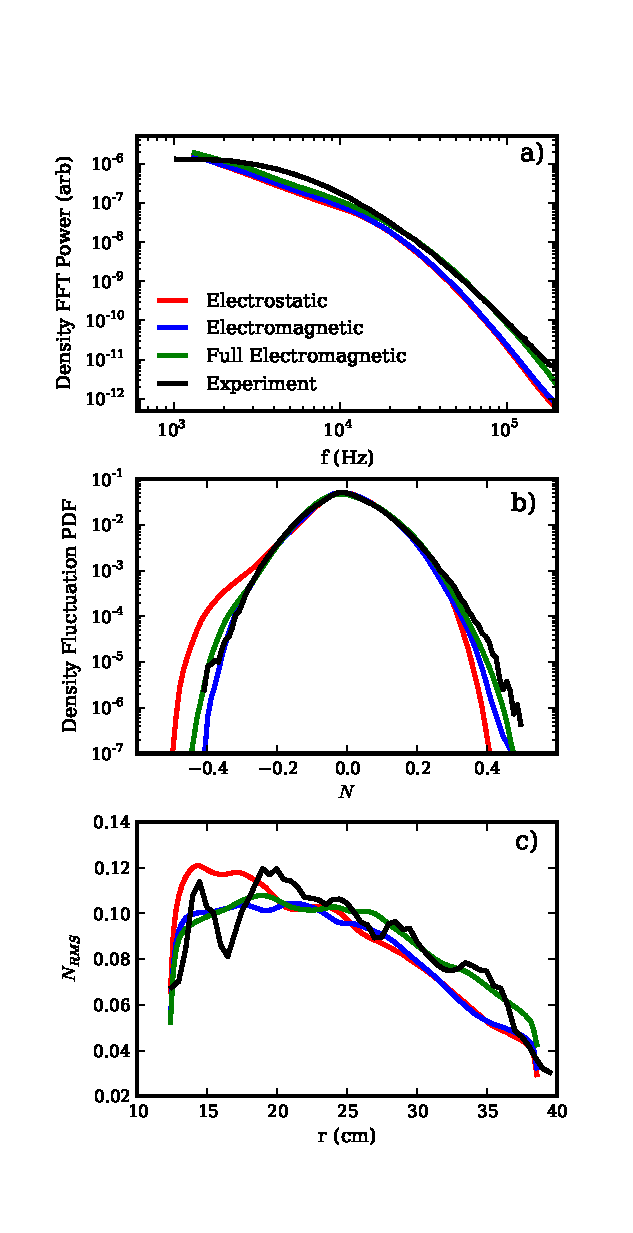
\includegraphics[]{es_vs_em_stats}
\hfil
\caption{Electromagnetic statistics comparison}
\label{es_vs_em_stats}
\end{figure}

Now, as mentioned above, we do not include any electromagnetic contributions in the simulations used in the following chapters. 
It seems rather unjustified to do so since we are clearly able to run electromagnetic simulations and they seem to reproduce experimental turbulence with slightly better accuracy 
than the electrostatic ones.
One justification for our abandonment of electromagnetic simulations, however, is that electromagnetic simulations take a bit longer than electrostatic ones due to the extra relation in Eq.~\ref{maxwell} 
that is used to solve for $A_\para$, which requires an inversion of the Laplacian. This takes extra computation. 
Another justification is that the electromagnetic equations make the energy dynamics analysis in Chapter~\ref{c_en_formalism} a bit more complicated. Both of these factors are mitigated, 
however, if the inertial term $n m_e \diff{\vpe}{t}$ is dropped. Nevertheless, at the beginning of this work, we strived to find the simplest possible model to describe the turbulence in LAPD,
and we determined that the electrostatic approximation was acceptable. At that time, we didn't have the results of Fig.~\ref{es_vs_em_stats}. If we had the time, we would redo all of the simulations
and analysis to include electromagnetic contributions, but drop the inertial term in Eq.~\ref{mom_eqn}. This is a clear route to take for future work. 
Nevertheless, we are confident that electromagnetics would not change any of our conclusions in this work.
So for the remainder of this work, we will present theoretical calculations, simulation results, and conclusions using the electrostatic approximation.
